\chapter{Ingeniería Inversa: la versión LM9} \label{cap:capitulo3_III}

La versión LM9 representa una actualización de la versión LM7, por lo que la mayoría de sus componentes ya son conocidos. Sin embrago, hay algunos cambios significativos que deben analizarse con profundidad, y que se describen a continuación.

\begin{enumerate}
	\item La principal diferencia con respecto a la versión anterior es que en este versión el software corre sobre una \textbf{arquitectura hardware distinta}. Ya no se utiliza una placa base de un PC industrial, sino que se corre sobre una \textbf{plataforma compuesta por una Raspberry Pi y un Arduino}. Mientras que la Raspberry Pi mantiene el sistema principal y el software, el Arduino controla los componentes hardware como el PGA, los LEDs y el LCD bajo las órdenes que recibe de la Raspberry.

	\item En el ámbito de análisis de sonido digital, se ha reemplazado la interfaz Open Sound System (\textbf{OSS}) por Advanced Linux Sound Architecture (\textbf{ALSA}). Para ello, todo el código relativo la captura de sonido desde las tarjetas de sonido y su interpretación ha tenido que re-implementarse, por lo que esta nueva versión provee una serie de clases y programas nuevos que debe estudiarse.

	\item Se ha ampliado al análisis espectral de sonido desde las 8 bandas del LM7 hasta las 31 de esta versión.

	\item Aunque en esta nueva versión se sigue haciendo un uso intensivo de ficheros, todos aquellos ficheros que hacían el papel de variables globales han sido reemplazadas por variables globales reales en memoria compartida. Para ello se ha creado un nuevo módulo al que han llamado \textit{SharedMemory}. Este módulo tiene como finalidad crear un segmento de memoria compartida de forma que otros programas puedan hacer uso de él.

	\item El LM9 dispone de dos micrófonos en lugar de uno.
\end{enumerate}

A diferencia de la versión anterior, \textbf{en esta versión solo disponemos de parte del código fuente} del limitador y de su hoja de especificaciones técnicas, y no del limitador físicamente. La conclusión de que el LM9 corre de una arquitectura nueva compuesta por una Raspberry Pi y un Arduino es resultado, nuevamente, del proceso de ingeniería inversa al que se ha sometido al código fuente del que se dispone. En él se ha podido encontrar algunos comentarios breves de los desarrolladores donde nombran al Arduino. Por parte de la Raspberry, se debe al uso de módulos Kernel en el script de arranque que tan solo existen o tienen sentido en una Raspberry. \\
Para detallar algo más, el código del que se dispone corresponde al que corre en la Raspberry. En este código no se incluye el de la aplicación web, como era el caso en el LM7, aunque se sabe con seguridad que hace uso de ella (así se indica en las especificaciones) y que ha sido actualizada, ya que se disponen de algunos scripts PHP que incluyen a otros desde el directorio raíz de Apache (\verb|/var/www|), los cuáles no existen en la versión del LM7.

\section{Comunicación entre Raspberry y Arduino} \label{sec:lms9-uart}
%\cite{termios} y \cite{fcntl}
La comunicación entre estos dos sistemas se realiza mediante un UART (Universal Aynchronous Receiver-Trasnmitter) con la ayuda de las librerías \verb|termios| y \verb|fcntl|. Conectados mediante el puerto serie, usan de interfaz de comunicación el fichero \verb|/var/slr/hardware/port| a una velocidad de transmisión (\textit{baud rate}) de 38400 bps. Para controlar el dispositivo, se utiliza la clase \verb|SerialPort|, la cual parece haber sido adaptada de un recurso online\footnote{\url{https://tldp.org/HOWTO/Serial-Programming-HOWTO/x115.html}}, sin demasiada modificación. Se puede ver al cabecera de esta clase en el código \ref{lst:lms9-serialport}

Mediante esta interfaz de comunicación el la Raspberry y el Arduino intercambian información y cooperan para mantener el funcionamiento del limitador. El Arduino, encargado de controlar los dispositivos hardware de más bajo nivel, parece funcionar simplemente como un orquestador; es el software que corre sobre la Raspberry quien realiza la toma de decisiones y se las comunica al Arduino mediante el UART para que las lleve a cabo. La comunicación es bidireccional, ya que el software también lee datos del Arduino para actualizar su estado interno. \\

\begin{lstlisting}[language=c++, caption={Clase SerialPort}, label={lst:lms9-serialport}]
#ifndef HH_SerialPort
#define HH_SerialPort

#include <stdio.h>
#include <unistd.h>	 //Used for UART
#include <fcntl.h>	 //Used for UART
#include <termios.h> //Used for UART

#define SerialPortError_NotOpen 1024
#define SerialPort_MaxDefaultReadBufferSize 1024

class SerialPort
{
private:
	int uartFd;

public:
	SerialPort();

	int Open(const char *portName, int baudRate);

	int Write(const char *string, int len = -1);

	int WriteLn(const char *string);

	int ReadString(char *output, int maxLength = SerialPort_MaxDefaultReadBufferSize);
};

#endif
\end{lstlisting}

\clearpage
\section{Arranque}

El arranque es bastante parecido al del LM7, aunque ya no se hace uso del servicio \verb|init.d|. Obviamente el script de arranque se ha tenido que adaptar para que pueda funcionar sobre una Raspberry, pero en general realiza las mismas tareas que el script de arranque de su predecesor. En este caso, el script de arranque lo podemos encontrar como parte del código fuente del software, dentro de la carpeta \verb|scripts/| y se llama \verb|StartUp|.

De entre todos los comandos que ejecuta el script de arranque (\ref{lst:lms9-init}) hay que llama especialmente la atención por la falta de consistencia (como viene siendo normal en el software de los LM), y es que se hace uso varias veces de las órdenes \verb|modprobe| y \verb|rmmod|, las cuales sirven respectivamente para cargar y descargar (en el sentido de ``eliminar'') módulos del kernel de Linux. Todos los módulos siguen por estándar una nomenclatura, letras minúsculas y palabras separadas por guiones, sin embargo en el script de arranque puede fácilmente detectarse que el módulo \verb|SoundCapturer| no sigue este estándar. Esto lleva a pensar que este módulo de kernel puede ser de implementación propia y específica para el LM9, quizás como driver para una tarjeta de sonido de fabricación personalizada, pero como no se dispone del limitador físico, no hay manera de confirmarlo y no puede dejar de ser una suposición. \\

\begin{lstlisting}[language=bash, caption={Script StartUp.}, label={lst:lms9-init}]
#!/bin/bash

ifconfig eth0 192.168.1.223 netmask 255.255.255.0
ifconfig eth1 192.168.1.223 netmask 255.255.255.0
route add -net default gw 192.168.1.1

echo "" >/tmp/mtab
mount /dev/mmcblk0p7 /var/slr
echo "Iniciando..." 2>/dev/null

PATH=/bin:/sbin:/usr/sbin:/usr/bin 2>/dev/null

modprobe snd-pcm-oss
modprobe snd-mixer-oss
modprobe SoundCapturer

# replace the ramdisk with the tmpfs for /var and /tmp
mkdir -p /tmp/log/nginx
mkdir -p /var/run/ssh
mkdir -p /tmp/run
mkdir -m 777 /tmp/tmp /tmp/php4 /tmp/php5 2>/dev/null
mount -o bind /tmp/php4 /var/lib/php4 2>/dev/null
mount -o bind /tmp/php5 /var/lib/php5 2>/dev/null
mkdir /tmp/channels

for interfaz in eth usb; do
    for i in $(seq 0 9); do
        ifconfig $interfaz$i:2 192.168.1.223 netmask 255.255.255.0
    done
done
route add -net default gw 192.168.1.1
/sbin/ifconfig lo 127.0.0.1 up 2>/dev/null
/sbin/route add -net 127.0.0.0 netmask 255.0.0.0 gw 127.0.0.1 dev lo 2>/dev/null

cd /lms/
./preparatoria
cd /

/usr/local/bin/ntpdate &
chmod 777 /var/slr/configuracion
chmod 777 /var/slr
chmod 777 /dev/*
chmod -R 777 /tmp
echo "" >/tmp/conf.tmp
chmod 777 /tmp/conf.tmp
echo "" >/tmp/cuVerified

# Modules
#rmmod snd_bcm2835 snd_soc_pcm512x_i2c snd_soc_tas5713 snd_soc_pcm512x snd_soc_pcm512x_i2c leds_gpio led_class
rmmod snd-usb-audio
rmmod SoundCapturer
modprobe SoundCapturer
modprobe snd-usb-audio

# Modulos a quitar
rmmod leds_gpio

# RTC Setup
modprobe i2c-dev
#modprobe rtc-pcf8563
modprobe rtc-ds1307
echo ds1307 0x68 >/sys/class/i2c-adapter/i2c-1/new_device
#echo ds3231 0x68 > /sys/class/i2c-adapter/i2c-1/new_device
#echo pcf8563 0x51 > /sys/class/i2c-adapter/i2c-1/new_device
hwclock -s

mkdir /tmp/sessions
mkdir /tmp/modules
chmod 777 /tmp/sessions /tmp/modules
mkdir -p /var/log/nginx/

service php5-fpm start &
service udev stop
service udev start &

# Register memory
chmod a+r /dev/mmcblk0p4

mkdir /var/run/sshd
service ssh restart &

/bin/runVersionCommands
\end{lstlisting}

\vspace{1em}

\begin{lstlisting}[language=bash, caption={Script runVersionCommands.}, label={lst:lms9-init}]
#!/bin/bash
#Adding a StartUp Log
fecha=$(date +%Y/%m/%d-%H:%M:%S)
echo "type=startUp&dni=noUser&name=noUser&time=$fecha&other=" >>/var/slr/logs.serial

echo -n "Hardware Service"
runHwController >/dev/null &
sleep 2
hardwareClient -input 1
sleep 1
hwUcWD >/dev/null &

echo " ...firstConfigs... "
LoadAudioDefaultPreset >/dev/null 2>/dev/null &
echo " Ok"

#Limiter services
echo -n "Limiter/Register services"
if getConfig | grep soundLevelLimiter; then
    echo "  Limiter:"
    echo "    HID type: Lcd and leds"
    #llControl >/dev/null 2> /dev/null &
    LcdControl &

    echo "Calibration control Service : "
    controlDeCalibracion >/dev/null 2>/dev/null &

    echo "Audio stream Services"
    runLines >/dev/null 2>/dev/null &
    runMicAnalyzer >/dev/null 2>/dev/null &

    echo "Register & Limiter"
    keepRg >/dev/null 2>/dev/null &
    keepLm >/dev/null 2>/dev/null &
else
    echo "  Limiter:"
    echo "    HID type: Lcd and leds"
    #panelControl >/dev/null 2> /dev/null &
    lcdControl &

    echo "Audio stream Services"
    runMicAnalyzer >/dev/null 2>/dev/null &

    echo "Register & Limiter"
    keepRg >/dev/null 2>/dev/null &
fi
echo " Ok"

echo -n "Audio stream keepers"
refreshAnalyzers >/dev/null 2>/dev/null &
Stabilyzer >/dev/null 2>/dev/null &
sleep 2
killall analyzer
echo " Ok"

echo -n "Network Services"
keepWebServer &
/var/slr/network.script >/dev/null 2>/dev/null
keepKnownIp >/dev/null 2>/dev/null &
keepComm >/dev/null 2>/dev/null &
#   /bin/adjtime >/dev/null 2> /dev/null &
in.telnetd -debug 1035 -L /bin/localservice &
remoteShellService >/dev/null &
echo "Ok"

echo -n "WatchDog services"
controlUptime &
\end{lstlisting}

\clearpage
\section{Detección de micrófono}

El micrófono, como el resto de de componentes hardware, está controlado por el Arduino, por lo que no se ha podido identificar el método de detección utilizado. El software recibe esta información mediante a interfaz de comunicación descrita en la sección \ref{sec:lms9-uart}. Para detectar si el micrófono está conectado o no se lee desde el dispositivo como si fuese un fuese un fichero, en el que se recibe un bloque de datos en formato JSON con el esquema \ref{lst:lms9-mic-detection}. Esta información se carga en la memoria compartida, quedando así disponible para el resto de programas del limitador. \\

\begin{lstlisting}[language=json, caption={Lectura del estado del micrófono en el LM9.}, label={lst:lms9-mic-detection}]
{
  "Status": {
    "type": "object",
    "properties": {
      "version": {
        "type": "string"
      },
      "ChannelPressure": {
        "type": "array",
        "minItems": 4,
        "maxItems": 4,
        "items": {
          "type": "number"
        }
      },
      "MicConnection": {
        "type": "boolean"
      },
      "InputPressure": {
        "type": "array",
        "minItems": 2,
        "maxItems": 2,
        "items": {
          "type": "number"
        }
      },
      "attenuation": {
        "type": "array",
        "minItems": 3,
        "maxItems": 3,
        "items": {
          "type": "number"
        }
      }
    }
  }
}
\end{lstlisting}



\clearpage
\section{Procesamiento de audio}

\begin{figure}[h]
    \centering
    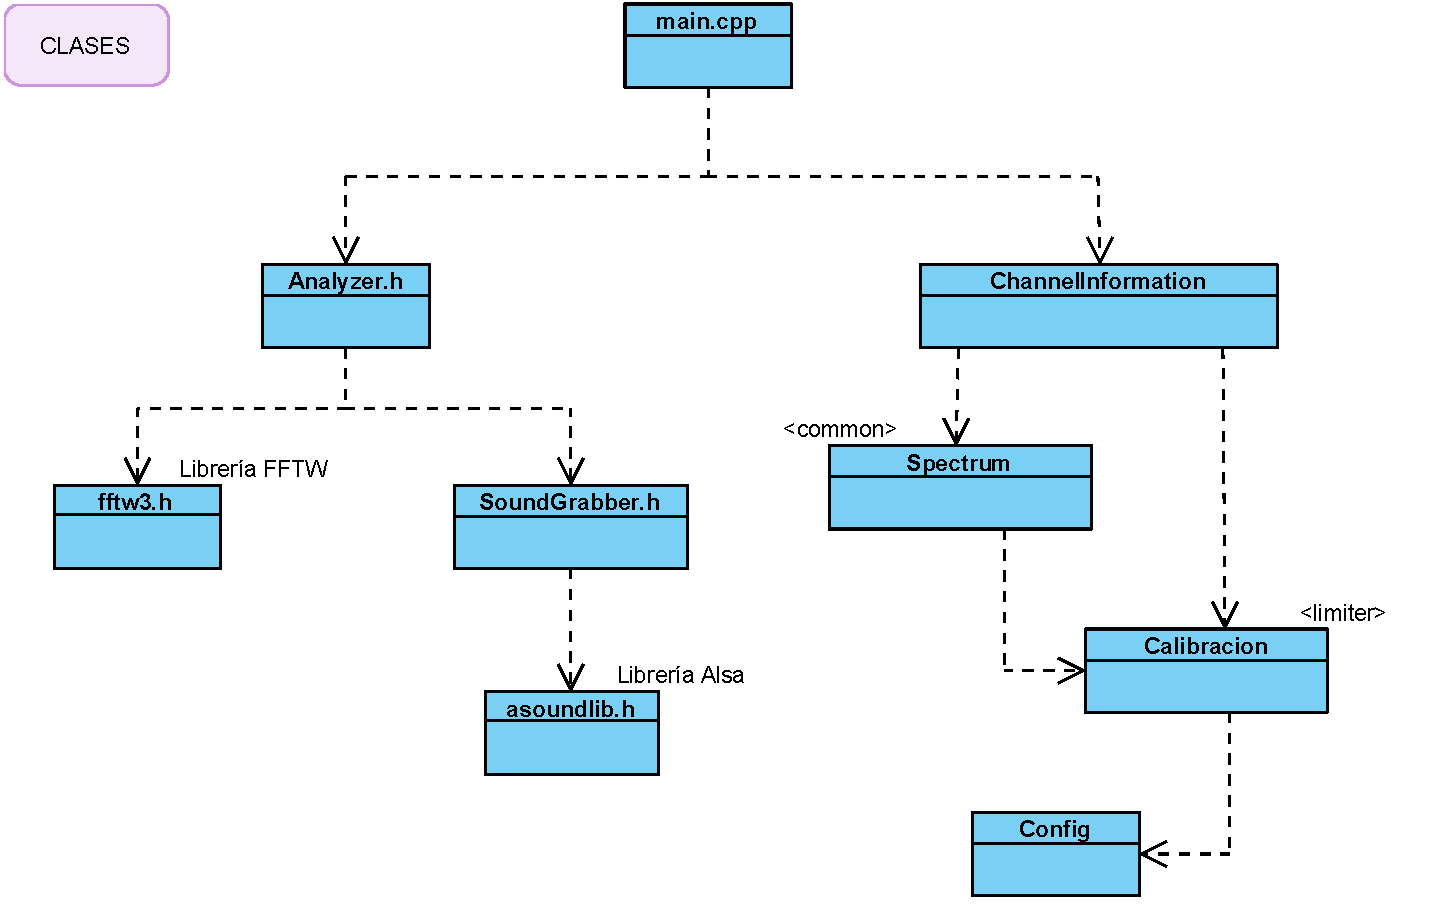
\includegraphics[width=0.9\textwidth]{figuras/lms9-analyzer.pdf}
    \caption{Diagrama de dependencias del módulo \texttt{Analyzer} en el LM9.}
    \label{fig:lm9-analyzer}
\end{figure}

Este módulo es con diferencia el gran cambio de esta nueva versión. Al pasar desde OSS a ALSA todo lo relacionado con el análisis del audio ha tenido que ser re-diseñado y re-escrito: La idea general sigue siendo la misma, se disponen de 2 tarjetas de sonido a las cuales nos conectamos mediante código para capturar y procesar el audio que por ellas transcurren, y mientras que una de las tarjetas nos proporciona la música procedente de la tabla de mezclas, la otra nos proporciona el audio procedente del micrófono instalado en la sala. De este modo tenemos las materias primas para poder generar los modelos necesarios y poder controlar tanto los niveles de emisión como los niveles de recepción.

El nuevo diseño se traduce en el desacople de funcionalidades desde una sola clase en el LM7 a varias en esta nueva versión. De este modo, se obtiene una estructura de clases ligeramente más compleja, pero más fácil de comprender ya dado que \textbf{cada clase tiene una única responsabilidad}, lo cual es buen principio de diseño (\textit{Principio de Responsabilidad Única}).

\subsection{Conexión a tarjetas de sonido}

\subsection{Interpretación de datos}

\subsection{Almacenamiento de audio}


\clearpage
\section{Gestión de calibración}

\subsection{Proceso de calibración}

El proceso de calibración se ha modificado ligeramente en esta nueva versión. De nuevo, no se tiene la certeza de cómo es exactamente el proceso de calibración ya que no disponemos del código de la interfaz web para esta versión, origen de este tipo de acciones, disparadas por el usuario.

El proceso de calibración bien podría ser exactamente igual que en el LM7, ya que el programa \verb|localservice| sigue existiendo en la misma versión y con las mismas capacidades en lo que al proceso de calibrado se refiere. Por otra parte, esta nueva versión proporciona un nuevo ejecutable llamado \verb|Calibrador|. Tras comparar los algoritmos de calibración de ambos programas podemos afirmar que, aunque con pequeñas diferencias en el código, el algoritmo de calibración implementado es el mismo. Sin embargo, este programa permite calibrar las líneas del limitador, pero no su micrófono, por tanto para este último caso debería seguir utilizándose la funcionalidad que proporciona \verb|localservice|. Sea como fuere, todo lo descrito en el proceso de calibración del LM7 (\ref{sec:lms7-calibrar}) puede aplicarse a esta versión.

\subsection{Ecualizaciones}

En el campo de las ecualizaciones se realizado ligeros cambios:
\begin{enumerate}
	\item Se ha añadido un nuevo vector por cada sensor (micrófono, línea derecha y línea izquierda), haciendo la distinción entre ecualización y ecualización interna.

	\item Todos los vectores son ahora de tamaño 31 (nº de bandas de frecuencias).
\end{enumerate}

La diferencia entre ecualización y ecualización interna viene dada por al ámbito de las mismas. Mientras que las ecualizaciones son definidas y configuradas por el usuario o instalador, las ecualizaciones internas son generadas de forma automática por el limitador durante el proceso de calibración, aunque también se permite su modificación manual.

\subsection{Emisión de ruido rosa}

La emisión de ruido rosa es una de la grandes incógnitas de esta versión, ya que no se ha encontrado nada al respecto en el código fuente, ni siquiera en la definición de órdenes para el Arduino. Como esta versión supone una actualización de la anterior, se puede suponer que la emisión de ruido rosa se realiza directamente desde la aplicación web, sin pasar por un proceso C++ del limitador. En la aplicación web del LM7 se invocan órdenes del sistema y procesos de forma directa con \verb|exec()| o \verb|popen()|, y de hecho existen funciones para controlar directamente las tarjetas de sonido y reproducir el fichero de ruido rosa. Sin otra alternativa, se ha de suponer que esto es así en esta versión y que la reproducción de ruido rosa se ha desacoplado de los procesos a bajo nivel del limitador.

Otra alternativa, la cual tendría más sentido teniendo en cuenta la arquitectura hardware vista en el LM7 (sección \ref{sec:lms7-pink}), sería que la emisión de ruido rosa estuviera controlada nuevamente por el Arduino. El software del limitador, de forma análoga a como se ha visto en otras secciones, ordenaría al Arduino la emisión de ruido rosa mediante el UART conectado al puerto serie. \\
Recordemos que en el LM7 una de las tarjetas de sonido reproduce de forma continua ruido rosa, pero solo obtiene un camino físico a la salida de audio del limitador cuando el conmutador (relé) se lo permite. Esto podría también ser así en esta versión, pero lo único que tenemos para poder al menos sospecharlo es la existencia de un comando en la interfaz de comunicación con el Arduino llamado \verb|noise|.

\subsection{Verificación: sesiones}

Este proceso no ha mostrado ningún cambio en su funcionamiento y sigue llevándose a cabo por el script PHP \verb|controlDeCalibracion|, sin embargo sí que ha introducido la generación y almacenamiento de un fichero en formato JSON con los datos de la última verificación realizada. Este fichero se almacena en la ruta \verb|/tmp/lastCalibrationTest.json|.

\subsection{Almacenamiento de calibraciones}

En este aspecto la versión actual no presenta ningún cambio con respecto a la versión LM7. Los ficheros de calibración se siguen almacenando en las mismas rutas y en formato binario.


\clearpage
\section{Gestión de la configuración}

El modelo de la configuración ha sufrido algunos cambios, mayormente limpieza de atributos importados desde la versión 7 que ya no son necesarios. A pesar de esto, toda la gestión de la configuración es idéntica a la versión anterior. La configuración se almacena y recupera de la misma manera y en los mismos ficheros que en la versión LM7, por lo que lo descrito en la sección \ref{sec:lms7-config} para la versión 7 es igualmente aplicable a esta versión.

Entre algunos de los cambios introducidos se encuentra la ampliación del vector de \textit{aislamiento} a 31 elementos, así como la creación de otro vector con nombre \textit{márgenes} con igual tamaño y tipo.

\subsection{Proceso de configuración}

Se ha añadido la capacidad de configurar el nuevo atributo \textit{márgenes}. El proceso de configuración en sí no presenta cambios respecto a la versión anterior. Véanse los anexos \ref{append:configurador} y \ref{append:F_conf.tmp} para más detalles.

\subsection{Almacenamiento de la configuración}

Sin cambios respecto a la versión LM7. Véase la sección \ref{sec:lms7-config} sobre el almacenamiento de la configuración en el LM7.

\clearpage
\section{Gestión de registros}

\subsection{Proceso de registro}

El proceso de registro ha sido llevado a un programa independiente, el \verb|Registrador|, por lo que la generación de registros ya no forma parte del programa \verb|Limitador|. Aún así, ahora ambos programas se ejecutan de forma ininterrumpida en paralelo. Aunque independiente, el algoritmo de registro de datos es idéntico al de la versión anterior, aunque ahora utilizad los datos que le proporciona el módulo \verb|Analyzer| y hace uso de las nuevas clases, así como de unas clases auxiliares para acumular los datos durante los 60 segundos que representa el registro. \\

\begin{lstlisting}[language=c++, label={lst:lms9-registrador}, caption={Generación de registros en el LM9.}]
	// Guardar registro
    if (time(NULL) - horaUltimoRegistro >= 60)
    {
      printf("Preparing to save\n");

      horaUltimoRegistro = time(NULL);
      if (ctr == 0)
        ctr = 1;

      estadoAGuardar = estado;
      estado.limpiaMascara();

      //Calculando medias
      printf("  Calculating averages (%d)\n", ctr);
      estadoAGuardar.mediaDeUnMinuto = micAccumulator / ctr;
      estadoAGuardar.presion = micAccumulator / ctr;
      estadoAGuardar.presionIzquierda = leftAccumulator / ctr;
      estadoAGuardar.presionDerecha = rightAccumulator / ctr;
      estadoAGuardar.recepcion = receptionAccumulator / ctr;

      //Creamos la media de las mediciones
      printf("  Spectrum averages (%d)\n", medicionesAcumulativas.ctr);
      medicionesAcumulativas.convertToAverage();
      medicionesAcumulativas.print();

      //Limpieza de valores acumulativos
      ctr = 0;
      micAccumulator = 0;
      leftAccumulator = 0;
      rightAccumulator = 0;
      receptionAccumulator = 0;

      //Creando el registro
      printf("  Creating registry entry\n");
      registro.crea(estadoAGuardar, configuracion);

      //mic,left,right;
      registro.setSpectrums(
          medicionesAcumulativas.mic.aWeighted,
          medicionesAcumulativas.left.aWeighted,
          medicionesAcumulativas.right.aWeighted);

      //Guardando registro
      if (!registrador.guardaRegistro(registro))
      {
        puts("Error al guardar registro");
      };
      registro.muestra();

      //Preparamos el objeto para recibir más datos
      medicionesAcumulativas.zero();
    }
\end{lstlisting}


\subsection{Almacenamiento de registros}

Los únicos cambios respecto a la versión anterior ha sido la adición de una matriz de datos de tipo flotante de tamaño [3][31] en la clase \verb|Registro|, para almacenar el espectro del micrófono y las líneas. El resto no ha presentado cambios. Para ampliar la información diríjase al anexo \ref{append:F_registro}.

\subsection{Lectura de registros}

Sin cambios respecto a la versión LM7. La lectura de los registros sigue realizándose mediante el uso del programa \verb|getData|. Puede ver el anexo \ref{append:getData} para completar la información.

\clearpage
\section{Proceso de atenuación}

\subsection{Comunicación con el PGA}

El PGA, como el resto de de componentes hardware, está controlado por el Arduino, de hecho ni siquiera queda completamente claro que exista en PGA, aunque todo parecer indicar que sí. El último paso del proceso de atenuación es comunicar la atenuación deseada al PGA, y en este caso, eso se traduce en comunicárselo al Arduino. La interfaz de comunicación con el Arduino ha quedado descrita en la sección \ref{sec:lms9-uart}. El programa \verb|limitador| escribe en el dispositivo la atenuación deseada tal y como se en el código \ref{lst:lms9-atenuacion}. \\

\begin{lstlisting}[language=c++, caption={Comunicación de la atenuación deseada en el LM9.}, label={lst:lms9-atenuacion}]
  // El arduino da la atenuación en negativo.
  char command[1024];
  sprintf(command, "echo max %.1f 10 10 %.1f 5 > /var/slr/hardware/port", -desiredAt, 0.0f);
  system(command);
\end{lstlisting}
